% při kompilaci dokumentu LuaLaTeXem dojde k chybě, protože
% nedefinuje \pdfpagewidth a \pdfpageheight. 
% Balíček luatex85 to napravuje
\ifdefined\directlua
\RequirePackage{luatex85}
\fi

\documentclass{csbulletin}
% \usepackage[T1]{fontenc}
% \usepackage[utf8]{inputenc}
\usepackage{fontspec}
\selectlanguage{czech}
\usepackage{luavlna}
\usepackage[noautomatic]{responsive}
\usepackage[all]{nowidow}
\usepackage{csquotes}

\usepackage{graphicx}
\usepackage{caption}
\usepackage{subcaption}


\usepackage[
  backend=biber,
  style=iso-numeric,
  sortlocale=cs,
  autolang=other,
  bibencoding=UTF8,
  mincitenames=2,
  maxcitenames=2,
]{biblatex}
\addbibresource{responsive.bib}
\usepackage[
  implicit=false,
  hidelinks,
]{hyperref}


\newcommand\balicek[1]{\textit{#1}}

\begin{document}

\title{Responzivní design s \LaTeX em}
\EnglishTitle{Responsive Design with \LaTeX}
\author{Michal Hoftich}
\podpis{Michal Hoftich, \url{michal.h21@gmail.com}}
\maketitle

\begin{abstract}
Tento článek se zaměřuje na použití metod responzivního designu pro zobrazení
webových stránek na zařízeních s různou velikostí displejů, jako jsou mobilní
telefony, tablety, velké monitory a tiskárny. Tyto metody umožňují optimalizaci
čitelnosti dokumentu na všech zařízeních pomocí použití různých velikostí
písma, jednotlivých prvků na stránce a okrajů.

Představíme způsob, jak lze podobné funkcionality dosáhnout
pomocí \LaTeX u. Konkrétně se zaměřuje na využití Lua\LaTeX u pro automatizovanou
sazbu s pomocí balíčků \balicek{Responsive} pro nastavení velikosti písma a řádkového prokladu
podle velikosti stránky, \balicek{Luavlna} pro zamezení výskytu jednopísmenných předložek
na koncích řádků, \balicek{Lua-widow-control} pro omezení osamocených řádků na koncích a
začátcích stránek a \balicek{Linebreaker}, který brání přetečení řádků.

Díky těmto metodám lze použít jeden zdrojový dokument pro různé výstupy, jako
jsou tiskové verze, čtečky e-knih a webové stránky, a dosáhnout optimálního
zobrazení dokumentu na všech zařízeních.
\end{abstract}
\klicovaslova: automatická sazba, responzivní design, Lua\LaTeX


\section{Úvod}

\begin{figure}[htbp]

  \centering
  \caption{Ukázka použití režimu \emph{zobrazení čtečky} v prohlížeči Firefox}

  \begin{subfigure}[t]{0.45\textwidth}
    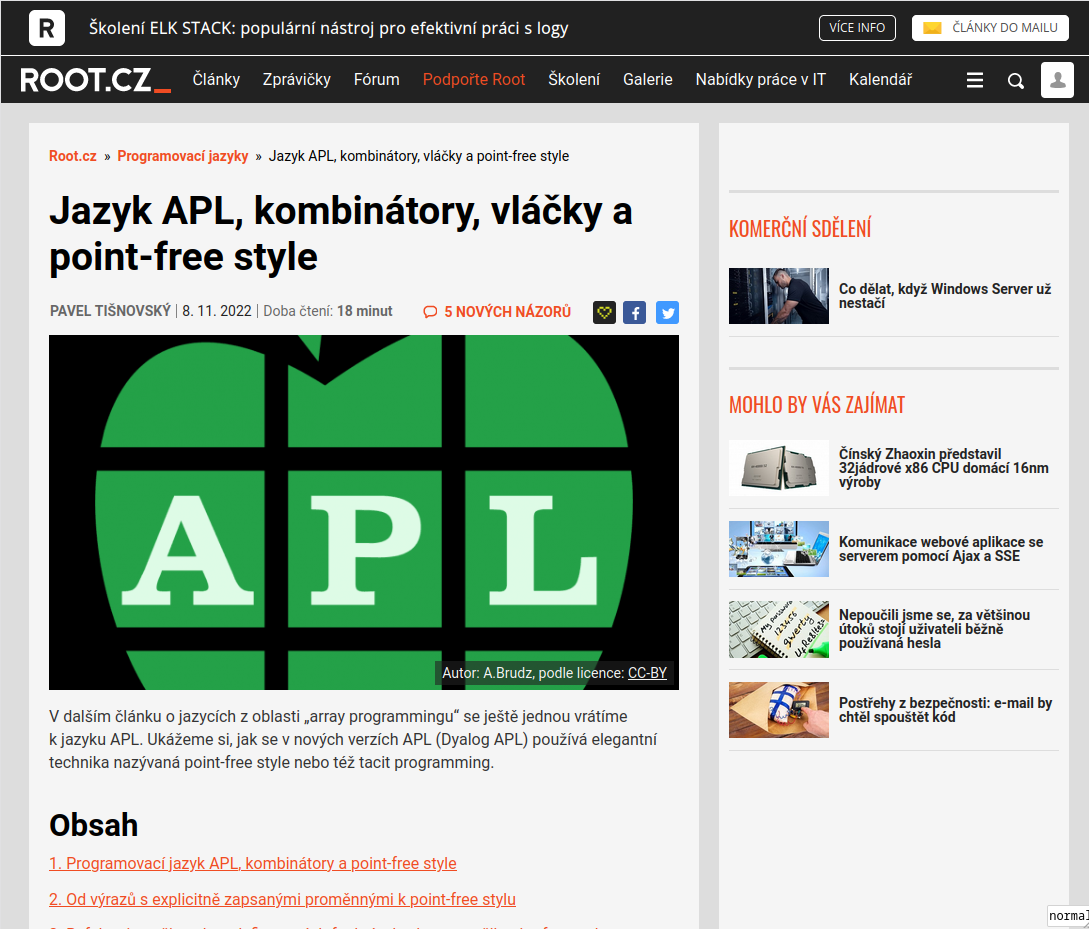
\includegraphics[width=\textwidth]{img/root-balast.png}
    \caption{Stránka s ovládacími prvky a reklamami}
  \end{subfigure}
  \hfill
  \begin{subfigure}[t]{0.45\textwidth}
    \includegraphics[width=\textwidth]{img/root-čtečka.png}
    \caption{Stránka v zobrazení čtečky}
  \end{subfigure}
\end{figure}



\begin{figure}[htbp]
\begin{subfigure}[t]{0.74\textwidth}
    
\includegraphics[width=\textwidth]{img/pedf-web-big.png}
    \caption{Ukázka stránky na velkém monitoru}
\end{subfigure}
\hfill
\begin{subfigure}[t]{0.24\textwidth}
    \includegraphics[width=\textwidth]{img/pedf-web-small.png}
    \caption{Ukázka stránky na malém displeji}
\end{subfigure}
\end{figure}

\begin{figure}[btbp]
  \caption{Nastavení velikosti písma podle velikosti displeje}

  % Velikost písma můžeme nastavit pomocí příkazu \verb|\setsizes{počet znaků na řádek}|.
  

\begin{verbatim}
\begin{minipage}{5cm}
\setsizes{25}

\lipsum[1]

\end{minipage}
\end{verbatim}
\fbox{%
\begin{minipage}{5cm}
\ResponsiveSetup{lineratio=38}
\setsizes{25}

\normalsize


Lorem ipsum dolor sit amet,
consectetuer adipiscing elit.
Ut purus elit, vestibulum ut,
placerat ac, adipiscing vitae,
felis. 

\end{minipage}}
\end{figure}

\printbibliography

\begin{summary}
  This article focuses on the use of responsive design techniques to display
  web pages on devices with different display sizes, such as mobile phones,
  tablets, large monitors and printers. These methods allow optimizing the
  readability of a document on all devices by using different font sizes,
  individual page elements, and margins.

  We present how similar functionality can be achieved using \LaTeX.
  Specifically, it focuses on the use of Lua\LaTeX{} for automated typesetting,
  using packages \balicek{Responsive} for setting font size and line spacing according to page size,
  \balicek{Luavlna} to prevent the occurrence of
  single-letter prepositions at line breaks, \balicek{Lua-widow-control} to
  reduce orphan lines at page breaks and page starts, and \balicek{Linebreaker}
  to prevent line overflow.

  With these methods, a single source document can be used for different
  outputs, such as print versions, e-book readers, and web pages, and achieve
  optimal document display on all devices.

\keywords: automatic typesetting, responsive design, Lua\LaTeX
\end{summary}
\end{document}
